\chapter{Sincronizzazione}
\section{Programmi concorrenti e sequenziali}
I programmi concorrenti hanno delle proprietà molto diverse rispetto ai più comuni programmi sequenziali con i quali i programmatori hanno maggiore familiarità.
\\Interazioni tra agenti concorrenti
\begin{description}
    \item[Cooperazione:] interazioni "prevedibili e desiderate". La loro presenza è necessaria per la logica del programma. Avviene tramite scambio di informazioni (anche semplici come segnali) - Sincronizzazione diretta o esplicita
    \item[Competizione:] gli agenti competono per accedere ad una risorsa condivisa. Politiche di accesso alla risorsa sono necessarie - Sincronizzazione può essere indiretta o implicita
    \item[Interferenze:] interazioni "non prevedibili e non desiderate" - errori di programmazione, spesso dipendenti dalle tempistiche (time dependent) e non facilmente riproducibili
\end{description}

\section{Meccanismi di sincronizzazione}
Sono i meccanismi che permettono di \underline{controllare l'ordine relativo delle varie attività dei processi/thread}.
\\Se \underline{modello di memoria condivisa}:
\begin{enumerate}
    \item \textbf{mutua esclusione}: dati, regioni critiche del codice, non sono accessibili contemporaneamente a più thread
    \item \textbf{sincronizzazione su condizione}: si sospende l'esecuzione di un thread fino al verificarsi di una opportuna condizione sulle risorse condivise
\end{enumerate}
Se \underline{modello a scambio di messaggi}:
\begin{itemize}
    \item di solito impliciti nelle primitive di \textit{send} e \textit{receive} == un thread può ricevere un messaggio solo dopo il suo invio
    \item \textbf{sincronizzazione su eventi}: si sospende l'esecuzione di un thread fino al verificarsi di un evento
\end{itemize}
Questi meccanismi vengono messi a disposizione dal sistema operativo nel caso di processi. In Java ritroviamo le stesse soluzioni implementate a livello di JVM per i thread.

\subsection{Sincronizzazione su eventi}
\subsubsection{Join}
\begin{itemize}
    \item Esempio di metodo per la sincronizzazione temporale di 2 thread
    \item Il metodo \verb#join# è definito nella classe Thread 
    \item Quando si invoca il metodo \verb#join()# su un thread, il thread chiamante entra in uno stato di attesa (wait). Rimane in tale stato finché il thread chiamato (t1) non termina
    \item Il metodo \verb#join()# può anche ritornare se il thread chiamato viene interrotto. In questo caso, il metodo lancia una \verb#InterruptedException#
    \item Infine, se il thread chiamato è già terminato o non è stato avviato, la chiamata al metodo \verb#join()# ritorna immediatamente
\end{itemize}
\begin{center}
    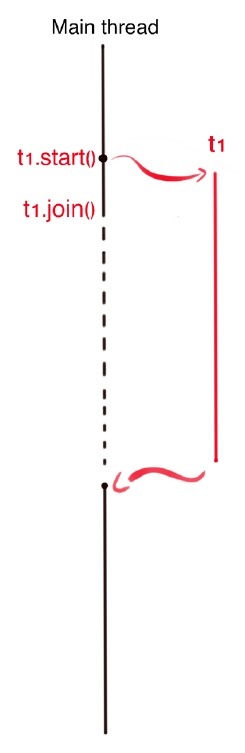
\includegraphics[width=0.75\textwidth]{img/sincronizzazione_join1.jpg}
\end{center}

\subsubsection{Barriere}
Meccanismo di sincronizzazione
\begin{itemize}
    \item I thread vengono messi progressivamente in attesa in attesa che una condizione globale non venga soddisfatta.
\end{itemize}
Esempio:
\begin{itemize}
    \item un compito comune suddiviso in più fasi e ogni fase è assegnata a più thread
    \item ogni thread esegue il suo task ed attende che tutti gli altri abbiano terminato prima di proseguire alla fase successiva
\end{itemize}
Possibile implementazione:
\begin{itemize}
    \item contatore condiviso conta il numero di processi che devono terminare
    \item il contatore decrementa ogni volta che un thread termina il suo task
    \item aggiornamento del contatore "atomico"
\end{itemize}
\begin{center}
    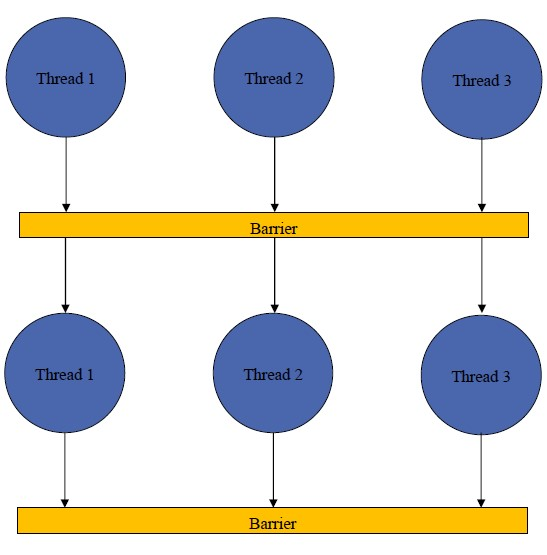
\includegraphics[width=0.75\textwidth]{img/sincronizzazione_barriere1.jpg}
\end{center}

\section{Problemi}
\subsection{Race condition}
\subsection{2}

\section{Come implementare la sincronizzazione}

\section{Come implementare la sincronizzazione}

\section{Come implementare la sincronizzazione}

\section{Come implementare la sincronizzazione}

